During the draft of the alloy, we omitted the aspects regarding the chain of custody because, as mentioned in Security description (3.7.3), these controls are made before storing information in the system, thus the other portions of the application are able to ignore it.

For this reason there is no constraint in Alloy that checks the fact that the report and the image can only exist if the information are genuine.
\newpage

\subsection{Alloy code}
\begin{figure}[!htbp]
	\centering
	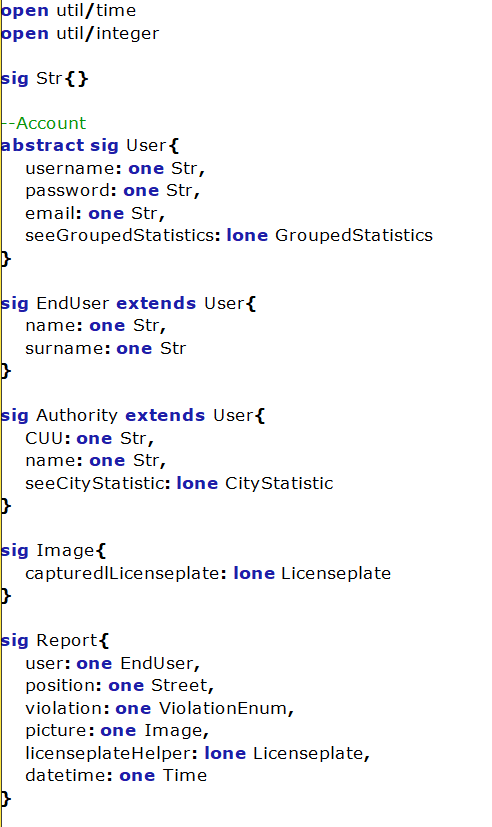
\includegraphics[width=0.9\linewidth, height=0.8 \textheight]{Images/Alloy/codealloy1}
	\caption{Signature 1}
	\label{Signature 1}
\end{figure}

\begin{figure}[h]
	\centering
	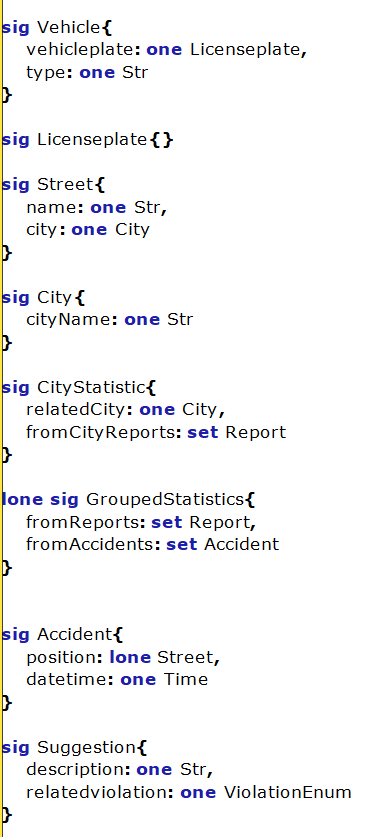
\includegraphics[width=0.5\linewidth, height=0.65\textheight]{Images/Alloy/codealloy2}
	\caption{Signature 2}
	\label{Signature 2}
\end{figure}

\begin{figure}[h]
	\centering
	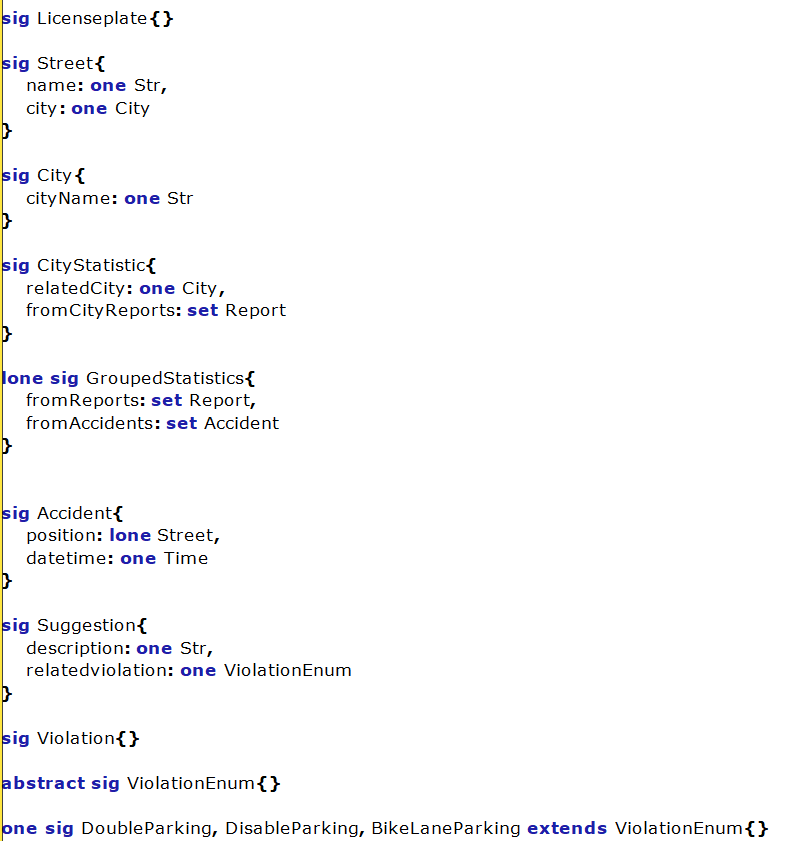
\includegraphics[width=0.9\linewidth, height=0.7\textheight]{Images/Alloy/codealloy3}
	\caption{Signature 3}
	\label{Signature 3}
\end{figure}

\begin{figure}[h]
	\centering
	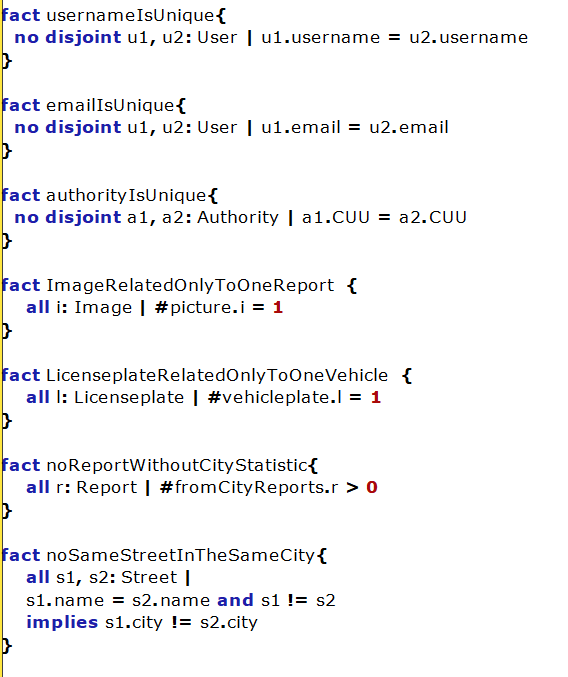
\includegraphics[width=0.9\linewidth, height=0.8\textheight]{Images/Alloy/codealloy4}
	\caption{Pred and Facts 1}
	\label{Pred and Facts 1}
\end{figure}

\begin{figure}[h]
	\centering
	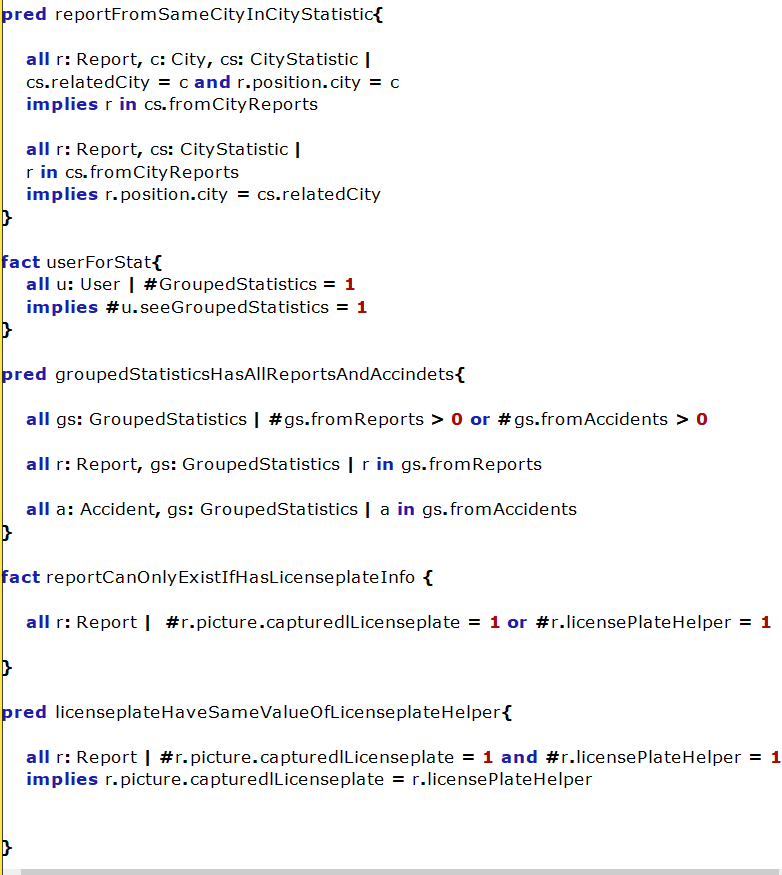
\includegraphics[width=0.9\linewidth, height=0.8\textheight]{Images/Alloy/codealloy5}
	\caption{Pred and Facts 2}
	\label{Pred and Facts 2}
\end{figure}

\begin{figure}[h]
	\centering
	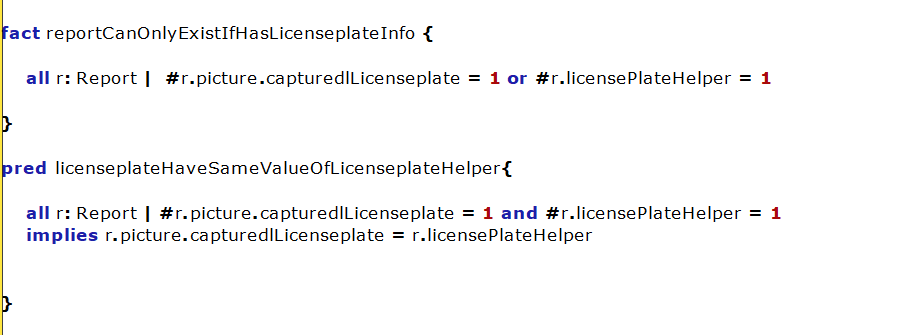
\includegraphics[width=0.9\linewidth, height=0.3\textheight]{Images/Alloy/codealloy6}
	\caption{Pred and Facts 3}
	\label{Pred and Facts 3}
\end{figure}

\begin{figure}[h]
	\centering
	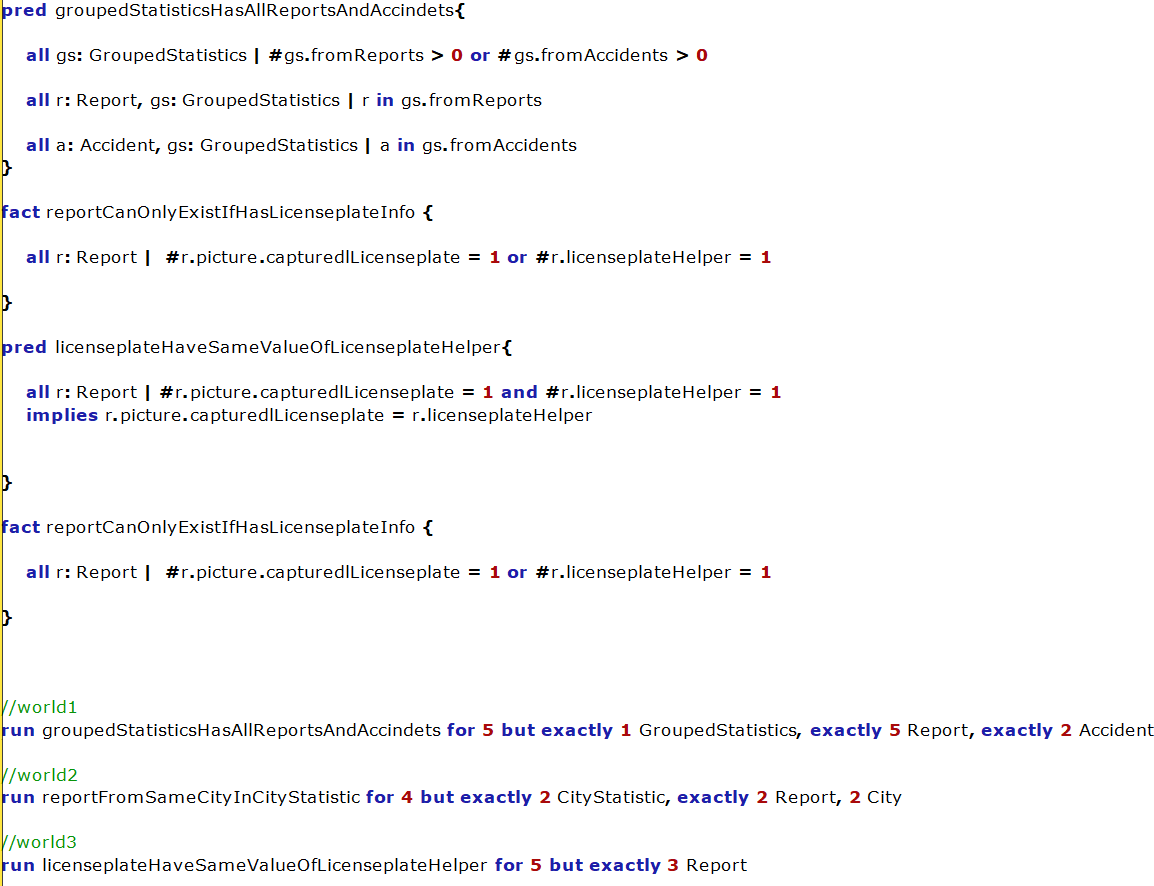
\includegraphics[width=0.95\linewidth, height=0.86\textheight]{Images/Alloy/codealloy7}
	\caption{Pred, Facts and World}
	\label{Pred and Facts and World}
\end{figure}
\FloatBarrier
\subsection{Predicates testing}
\subsubsection{World 1}
Predicate about the aggregation of data coming from reports with the traffic information.

This predicate describes the constraint that the signature that represent statistics can only exist if and only if there is at least one report or accident.
Furthermore all reports and all accidents must be related to statistics.
\begin{figure}[h]
	\centering
	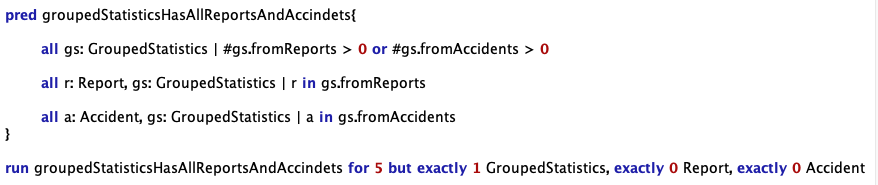
\includegraphics[width=0.9\linewidth, height=0.15\textheight]{Images/Alloy/test-world11}
	\caption{Pred 1}
	\label{Pred 1}
\end{figure}
\FloatBarrier
To show that the predicate works as expected, we have run the predicate with with inconsistent number of sig entities: exactly of  0 reports and 0 accidents but 1 GroupedStatistic
\begin{figure}[h]
	\centering
	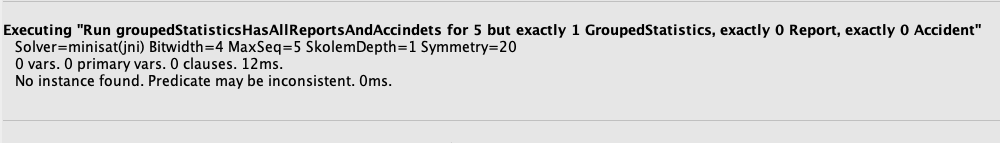
\includegraphics[width=0.9\linewidth, height=0.12\textheight]{Images/Alloy/test-world12}
	\caption{Result pred 1}
	\label{Result pred 1}
\end{figure}
\FloatBarrier
\newpage
The following represented world is generated from the following run: run groupedStatisticsHasAllReportsAndAccindets for 5 but exactly 1 GroupedStatistics, exactly 5 Report, exactly 2 Accident
\begin{figure}[h]
	\centering
	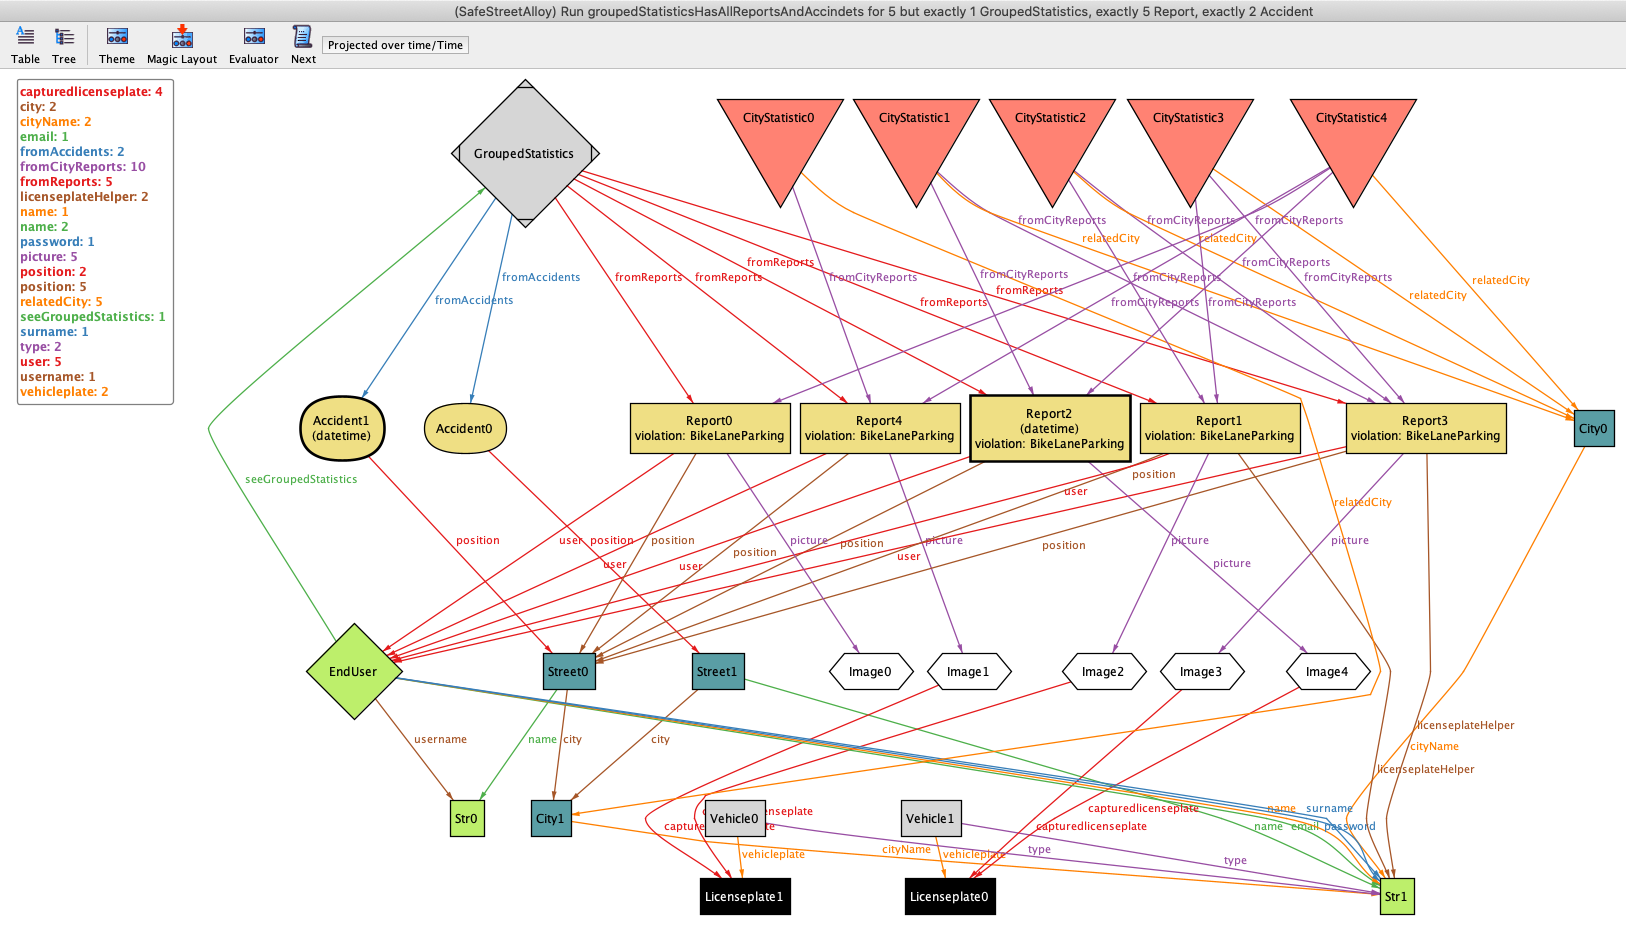
\includegraphics[width=0.9\linewidth, height=0.5\textheight]{Images/Alloy/world1}
	\caption{World 1 generated by pred 1}
	\label{World1 }
\end{figure}
\FloatBarrier
\newpage
\subsubsection{World 2}
Consistency between city and statistics.

This predicate describes the constraint that the signature that represent statistics specific about a city and all reports about all streets of the city must be related.
\begin{figure}[h]
	\centering
	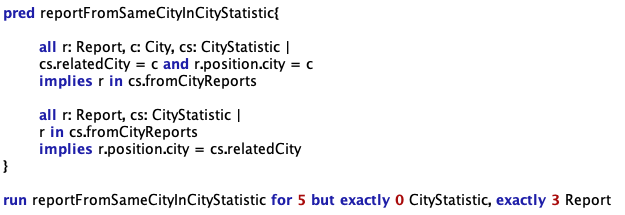
\includegraphics[width=0.9\linewidth, height=0.15\textheight]{Images/Alloy/test-world21}
	\caption{Pred 2}
	\label{Pred 2}
\end{figure}
\FloatBarrier
To show that the predicate works as expected, we have run the predicate with with inconsistent number of sig entities: exactly 0 CityStatistic, exactly 3 Report.
\begin{figure}[h]
	\centering
	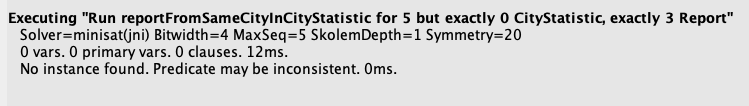
\includegraphics[width=0.9\linewidth, height=0.11\textheight]{Images/Alloy/test-world22}
	\caption{Result pred 2}
	\label{Result pred 2}
\end{figure}
\FloatBarrier
\newpage
The following represented world is generated from the following run: run reportFromSameCityInCityStatistic for 4 but exactly 2 CityStatistic, exactly 2 Report, 2 City
\begin{figure}[h]
	\centering
	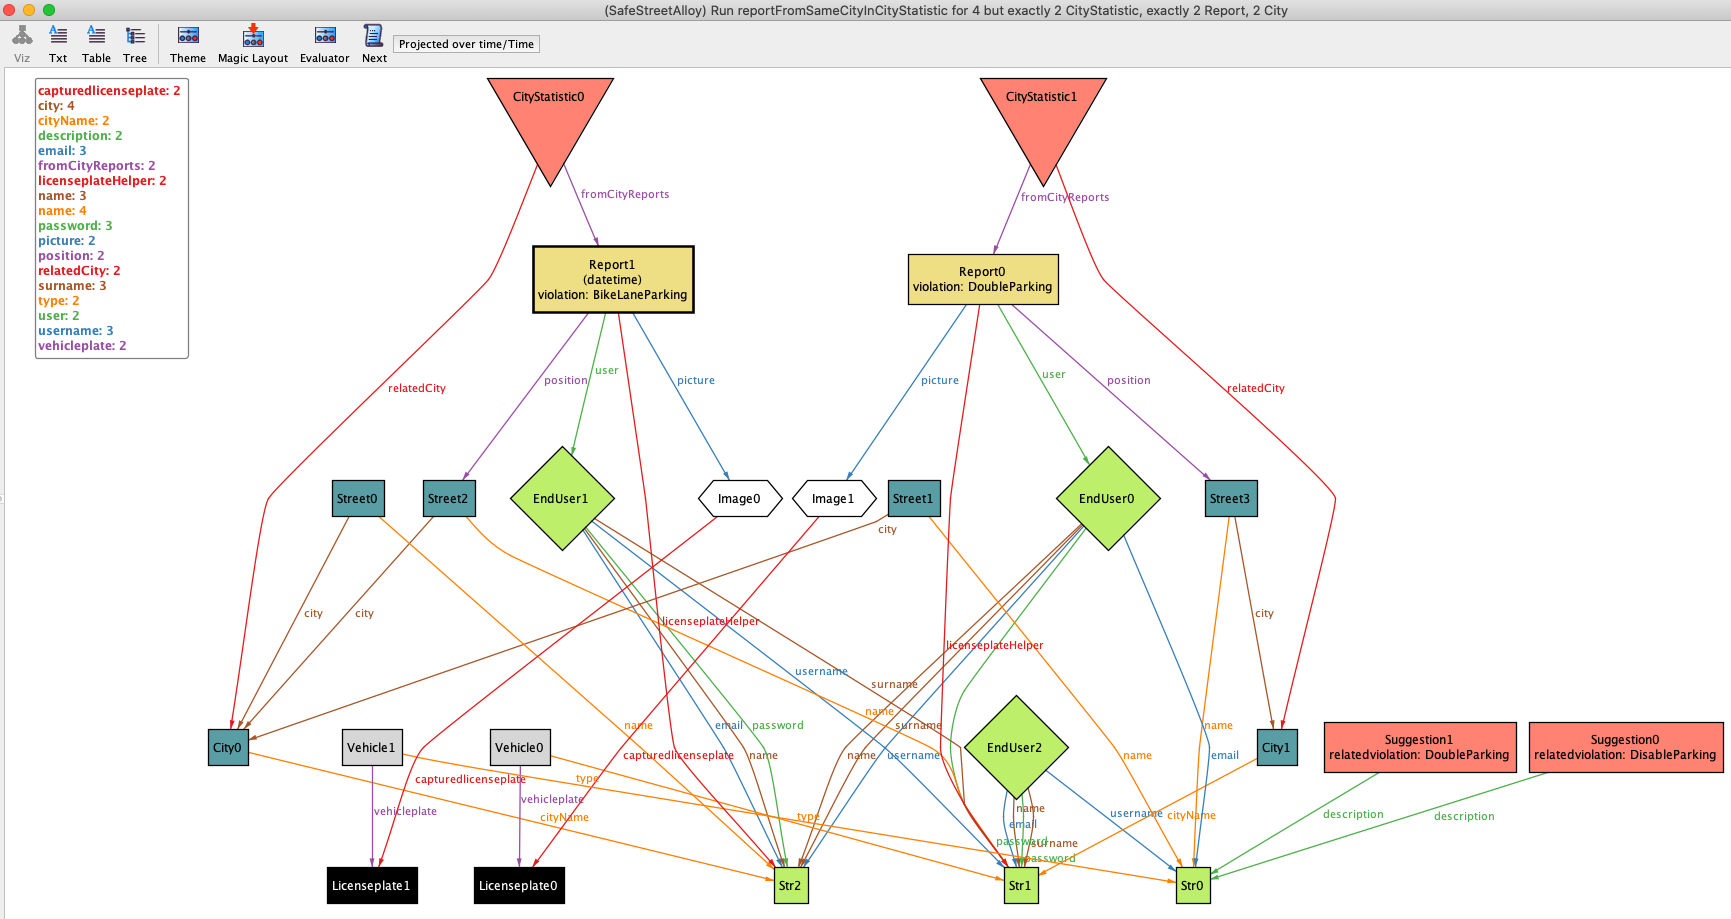
\includegraphics[width=1\linewidth, height=0.47\textheight]{Images/Alloy/world2}
	\caption{World 2}
	\label{World2}
\end{figure}
\FloatBarrier
\newpage
\subsubsection{World 3}
Predicate that test if the licenseplate retrieve from SafeStreets is the same suggested by the user.
\begin{figure}[h]
	\centering
	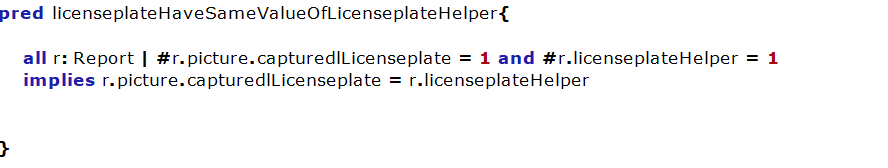
\includegraphics[width=0.9\linewidth, height=0.15\textheight]{Images/Alloy/predworld31}
	\caption{Predicate 3}
	\label{Pred 3}
\end{figure}

\begin{figure}[h]
	\centering
	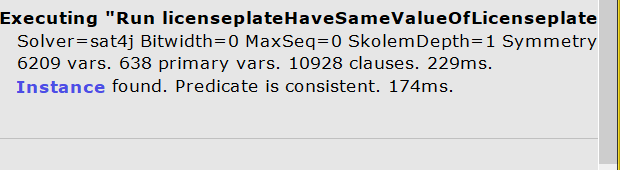
\includegraphics[width=0.8\linewidth, height=0.11\textheight]{Images/Alloy/predworld32}
	\caption{Result pred 3}
	\label{Result pred 3}
\end{figure}
\FloatBarrier
\newpage
The following represented world is generated from the following run: run licenseplateHaveSameValueOfLicenseplateHelper for 5 but exactly 3 Report
\begin{figure}[h]
	\centering
	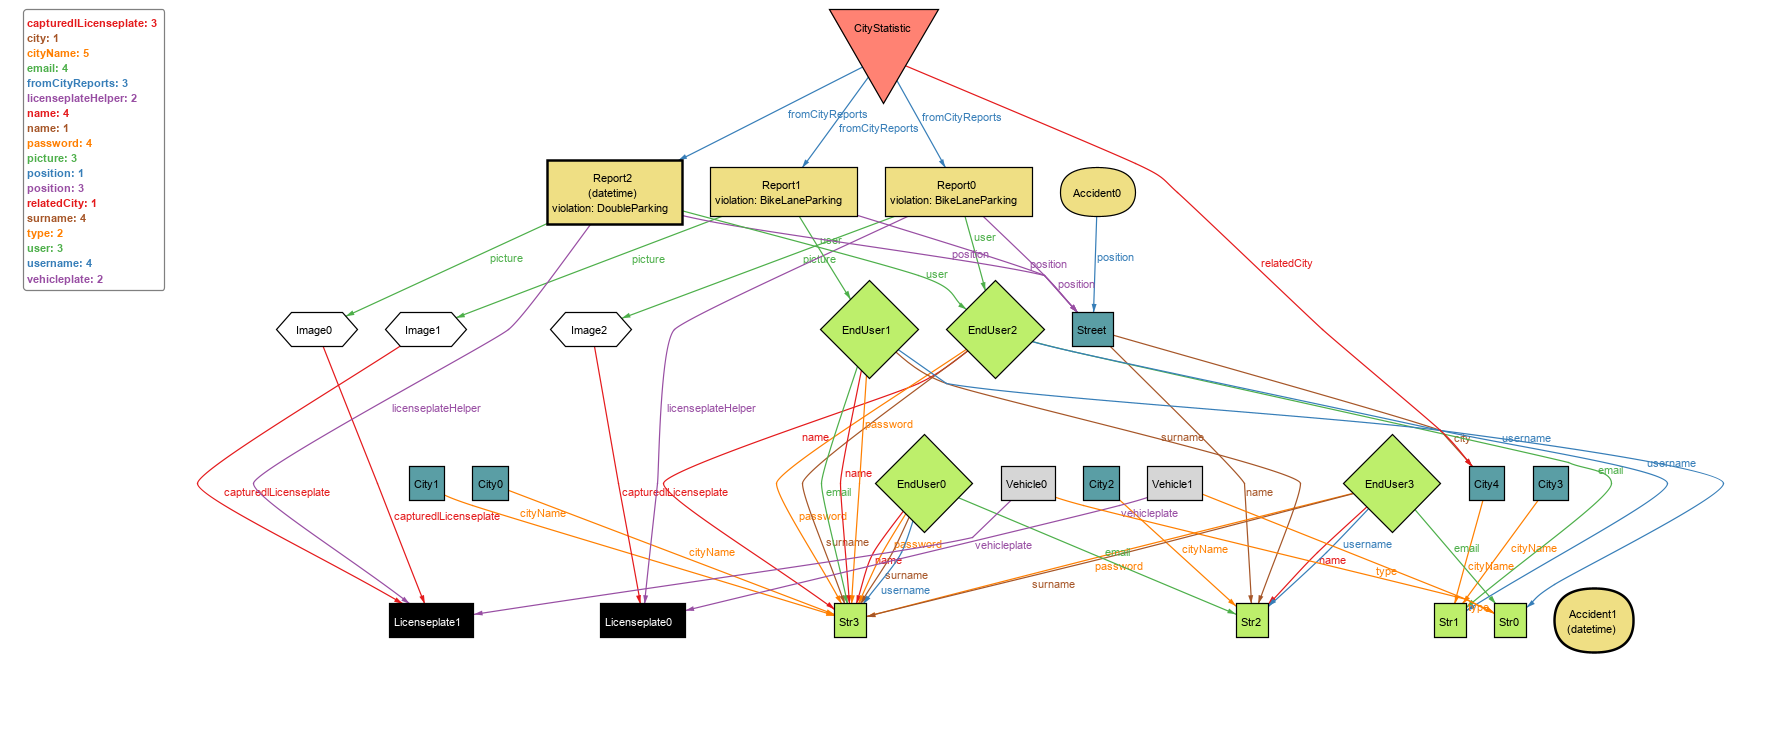
\includegraphics[width=1.1\linewidth, height=0.55\textheight]{Images/Alloy/world3alloy}
	\caption{World 3}
	\label{World3}
\end{figure}
